\documentclass[t,usenames,dvipsnames]{beamer}
\usetheme{Copenhagen}
\setbeamertemplate{headline}{} % remove toc from headers
\beamertemplatenavigationsymbolsempty

\usepackage{amsmath, sfmath, tikz, xcolor, pgfplots, array}
\pgfplotsset{compat = 1.16}
\usetikzlibrary{arrows.meta, calc, decorations.pathreplacing}

\title{Graphs of Sine and Cosine}
\author{}
\date{}

\AtBeginSection[]
{
  \begin{frame}
    \frametitle{Table of Contents}
    \tableofcontents[currentsection]
  \end{frame}
}

\begin{document}

\maketitle



\begin{frame}{Intro}
We can graph the sine and cosine functions in the same manner we can graph any function: by plotting points and then connecting them.    \newline\\ \pause

If we let the $x$-coordinates represent the measure of the angle and let the $y$-coordinates represent the value of the ratio, we can plot the graph of the sine function.
\end{frame}

\begin{frame}{Sine Graph}
\begin{center}
    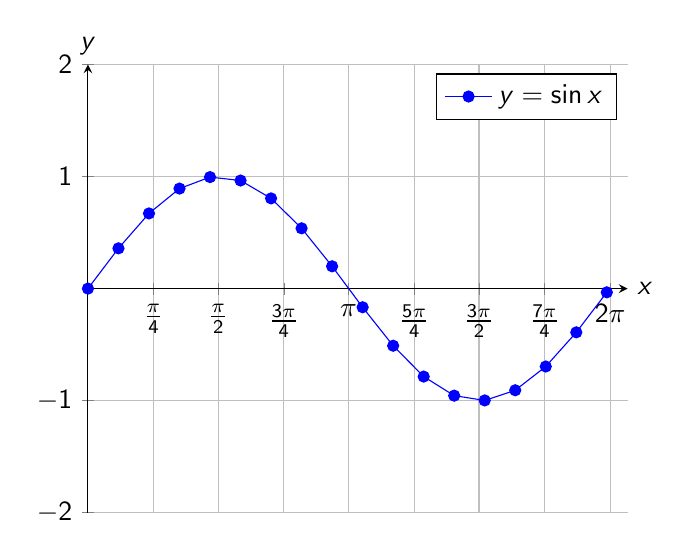
\begin{tikzpicture}
    \begin{axis}[
    axis lines = middle,
    xmin = 0, xmax = 6.5,
    ymin = -2, ymax = 2,
    grid, domain=0:6.25,
    xtick = {0, 0.79, 1.57, 2.36, 3.14, 3.93, 4.71, 5.50, 6.29},
    xticklabels = {0, $\tfrac{\pi}{4}$, $\tfrac{\pi}{2}$, $\tfrac{3\pi}{4}$, $\pi$, $\tfrac{5\pi}{4}$, $\tfrac{3\pi}{2}$, $\tfrac{7\pi}{4}$, $2\pi$},
    xlabel = $x$, 
    xlabel style={at=(current axis.right of origin), anchor=west},
    ylabel = $y$,
    ylabel style={at=(current axis.above origin), anchor=south}
    ]
    \addplot [mark = *, color=blue, samples = 18] {sin(deg(x))};
    \addlegendentry{$y=\sin x$};
    \end{axis}
    \end{tikzpicture}
\end{center}
\end{frame}

\section{Find the Amplitude of a Sine or Cosine Function}

\begin{frame}{Amplitude}
The \alert{amplitude} of a sine or cosine function is 
\[
\frac{1}{2}\left(\text{Maximum} - \text{Minimum}   \right)
\]
\pause
In the graph previously, the maximum of the graph is 1. The minimum of the graph is $-1$. Thus, the amplitude of $y=\sin x$ is
\[
\frac{1}{2}\left(1 - (-1)\right) = 1
\]
\end{frame}

\begin{frame}
If we want to change the amplitude, we need to \textbf{stretch the graph vertically}. Recall that vertical stretches involve multiplying the function by a positive value (negative values reflect the graph across the $x$-axis).  \newline\\   \pause

For functions in the form
\[
y = A\sin x \qquad \text{or} \qquad y = B\cos x
\]
the amplitude is $|A|$.
\end{frame}

\begin{frame}{Example 1}
Determine the amplitude of each of the following.   \newline\\
(a) \quad $y = 3\sin x$ \pause
\[
\text{Amplitude} = |3| = 3
\]
\pause
(b) \quad $y = 5.5\sin x$   \pause
\[
\text{Amplitude} = |5.5| = 5.5
\]
\pause
(c) \quad $y = 0.5\cos x$   \pause
\[
\text{Amplitude} = |0.5| = 0.5
\]
\pause
(d) \quad $y = -2\cos x$    \pause
\[
\text{Amplitude} = |-2| = 2
\]
\end{frame} 

\section{Determine the Period of a Sine or Cosine Function}

\begin{frame}{Period}
The graphs of sine and cosine are \textbf{periodic}, in that the pattern repeats itself infinitely in both directions. The graph of $y = \cos x$ is shown below.    \newline\\ 

\begin{center}
    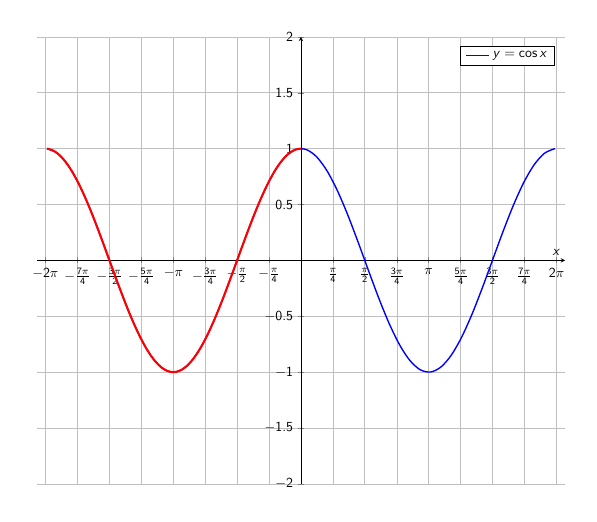
\begin{tikzpicture}[scale=0.5]
    \begin{axis}[
    axis lines = middle,
    xmin = -6.5, xmax = 6.5,
    ymin = -2, ymax = 2,
    grid, domain=-6.25:6.25,
    width = 15cm,
    xtick = {-6.29, -5.5, -4.71, -3.93, -3.14, -2.36, -1.57, -0.79, 0, 0.79, 1.57, 2.36, 3.14, 3.93, 4.71, 5.50, 6.29},
    xticklabels = {$-2\pi$, $-\tfrac{7\pi}{4}$, $-\tfrac{3\pi}{2}$, $-\tfrac{5\pi}{4}$, $-\pi$, $-\tfrac{3\pi}{4}$, $-\tfrac{\pi}{2}$, $-\tfrac{\pi}{4}$, 0, $\tfrac{\pi}{4}$, $\tfrac{\pi}{2}$, $\tfrac{3\pi}{4}$, $\pi$, $\tfrac{5\pi}{4}$, $\tfrac{3\pi}{2}$, $\tfrac{7\pi}{4}$, $2\pi$},
    xlabel = $x$
    ]
    \addplot [color=blue, line width = 1, samples = 50, smooth] {cos(deg(x))};
    \addplot [color=red, line width = 1.5, samples=50, smooth, domain=-6.25:0] {cos(deg(x))};
    \addlegendentry{$y=\cos x$};
    \end{axis}
    \end{tikzpicture}
\end{center}
\end{frame}

\begin{frame}{Period}
Notice that the part of the graph in purple is a copy of the part of the graph in blue. This is because the cosine function is \alert{periodic}.   \newline\\   \pause

Each of the following are ways in which you can think of the period of the graph of a function:   \pause  \newline\\
\begin{itemize}
    \item How long until the graph starts to repeat the same values in the same order.  \pause  \newline\\
    \item What is the least amount of the graph you would need to copy to paste it before and after the copy?   \pause  \newline\\
    \item If the units along the $x$-axis were length, period would be the wavelength from science class.
\end{itemize}
\end{frame}

\begin{frame}{Changing the Period}
We can adjust the period of the sine and cosine functions by multiplying the input values, $x$, by a positive number other than 1. \newline\\    \pause

Thus, the equation for adjusting the period of sine and cosine functions is
\[
y = \sin (Bx) \quad \text{ and } \quad y = \cos (Bx)
\]
\end{frame}

\begin{frame}{Example 2}
Use a graphing utility to determine the period of each of the following.   \newline\\  
(a) \quad $y = \sin(2x)$    \newline\\ \pause
Period = $\pi$    \vspace{12pt}  \newline\\ \pause
(b) \quad $y = \cos(3x)$    \newline\\ \pause
Period = $\frac{2\pi}{3}$
\end{frame}

\begin{frame}{Example 2}
(c) \quad $y = \sin \left(\frac{1}{2} x\right)$ \newline\\  \pause
Period = $4\pi$    \vspace{12pt}  \newline\\ \pause
(d) \quad $y = \cos \left(\frac{1}{4} x\right)$ \newline\\  \pause
Period = $8\pi$
\end{frame}

\begin{frame}{Period}
With $y = \sin(Bx)$ and $y = \cos(Bx)$, looking at the graphs, it would seem that the different values of $B$ affect the graphs in different ways.    \newline\\  \pause 

Notice in each case, our answers are whatever $2\pi / B$ equals. \newline\\ \pause

Therefore, the period of the graph of the sine and cosine functions is
\[
\frac{360^\circ}{B} \quad \text{or} \quad \frac{2\pi}{B}
\]
\end{frame}


\section{Determine the Vertical Shift of a Sine or Cosine Function}

\begin{frame}{Vertical Shifts}
Recall from transforming functions that we shift functions vertically by adding or subtracting a value \emph{from the function itself}.   \newline\\ \pause

For sine and cosine functions, the vertical shift becomes
\[
y = \sin x + D  \quad   \text{ and }    \quad   y = \cos x + D
\]
\end{frame}

\begin{frame}{Example 3}
Determine the vertical shift for each of the following.  \newline\\
(a) \quad $y = \sin x + 3$  \newline\\ \pause
Vertical shift = Up 3 units \newline\\ \pause
(b) \quad $y = \cos x - 1$ \newline\\ \pause
Vertical shift = Down 1 unit
\end{frame}

\begin{frame}{Example 3}
(c) \quad $y = 2\sin x - 4$ \newline\\ \pause
Vertical shift = Down 4 units   \newline\\  \pause
(d) \quad $y = -0.5\cos x$  \newline\\  \pause
Vertical shift = None (or 0 units)
\end{frame}

\section{Determine Phase Shifts of a Sine or Cosine Function}

\begin{frame}{Phase Shifts}
In trigonometry, phase shifts are the periodic functions' version of \alert{horizontal shifts}.  \newline\\  \pause

For sine and cosine functions, phase shifts typically resemble the following:
\[
y = \sin (Bx - C) \quad \text{ and } \quad y = \cos (Bx - C)
\]
\end{frame}

\begin{frame}{Phase Shifts}
To find the value of the phase shift, set $Bx-C=0$ and solve.   \newline\\ \pause

This value will be how far from the origin your graph shifts: \newline\\  \pause
\begin{itemize}
    \item Positive answer: shifts right \newline\\  \pause
    \item Negative answer: shifts left
\end{itemize}
\end{frame}

\begin{frame}{Example 4}
Determine the phase shift of each of the following. Don't forget to indicate direction. \newline\\
(a) \quad $y = \sin\left(x-\dfrac{\pi}{6}\right)$  \pause
\begin{align*}
    \onslide<2->{x-\frac{\pi}{6} &= 0} \\[10pt]
    \onslide<3->{x &= \frac{\pi}{6}} \\[10pt]
\end{align*}
\onslide<4->{The graph is shifted $\dfrac{\pi}{6}$ to the right.}
\end{frame}

\begin{frame}{Example 4}
(b) \quad $y = \cos\left(x+\dfrac{3\pi}{4}\right)$ \pause
\begin{align*}
    \onslide<2->{x+\frac{3\pi}{4} &= 0} \\[10pt]
    \onslide<3->{x &= -\frac{3\pi}{4}}  \\[10pt]
\end{align*}
\onslide<4->{The graph is shifted $\dfrac{3\pi}{4}$ to the left}
\end{frame}

\begin{frame}{Example 4}
(c) \quad $y = \sin\left(2x+\dfrac{\pi}{2}\right)$ \pause
\begin{align*}
    \onslide<2->{2x+\frac{\pi}{2} &= 0} \\[10pt]
    \onslide<3->{2x &= -\frac{\pi}{2}} \\[10pt]
    \onslide<4->{x &= -\frac{\pi}{4}}  \\[10pt]
\end{align*}
\onslide<5->{The graph is shifted $\dfrac{\pi}{4}$ to the left}
\end{frame}

\begin{frame}{Example 4}
(d) \quad $y = \cos\left(3x-\dfrac{3\pi}{2}\right)$ \pause
\begin{align*}
    \onslide<2->{3x-\frac{3\pi}{2} &= 0} \\[10pt]
    \onslide<3->{3x &= \frac{3\pi}{2}} \\[10pt]
    \onslide<4->{x &= \frac{\pi}{2}}    \\[10pt]
\end{align*}
\onslide<5->{The graph is shifted $\dfrac{\pi}{2}$ to the right}
\end{frame}

\begin{frame}{Summary}

\begin{center}
For $y = A\sin\left(Bx-C\right) + D$ \quad or \quad $y=A\cos\left(Bx-C\right) + D$: \\[18pt]

\setlength{\extrarowheight}{11pt}
\begin{tabular}{|c|c|c|c|}
    \hline
    \textbf{Amplitude}  &   \textbf{Period} &   \textbf{Phase Shift}  &   \textbf{Vertical Shift} \\[6pt] \hline
    $|A|$ &   $\dfrac{360^\circ}{B}$ or $\dfrac{2\pi}{B}$ &   $\dfrac{C}{B}$  &   $D$ \\[11pt] \hline
\end{tabular}
\end{center}
\end{frame}


\end{document}
